%% Benjamin Williams <bwilliams@lincoln.ac.uk>
%% Get in touch if you have any questions or problems!
%% University of Lincoln Computer Science Thesis Template

%% @version     1.0.4
%% @lastchanged 12th June 2020

% The document class -- remove [harvard] if you want
% numeric-style referencing.
\documentclass[harvard]{lincolncsthesis}

% Custom packages that you need to include
% Packages you intend to use
% ..

% For example, if you want to render 
% the document in a different font you can
% use something like: 

% \usepackage{gentium}

\usepackage{url}
\usepackage{amssymb}
\usepackage{amsmath}

% Your thesis details -- edit the file at the path below
% so it shows your name, title, etc. 
% Put the correct details in here
\author{Benjamin Williams}
\thesisDegree{Doctor of Philosophy}
\thesisSubmissionDate{July 2019}

% If your thesis title spans over three lines, prepend the command with \Large!
\title{\bfseries Your Thesis Title}

% Supervisor details
\thesisSupervisor{Dr. Mantis Toboggan}

% Set up the bib files which are gonna be used
% throughout this document
% Add in the .bib files you wish to add 
% into your document here. If you want to
% include others, just copy this line and
% change the path!

\addbibresource{bib/references.bib}


% This thesis template also supports rendering
% a ludography. To cite games, make sure your reference
% in your bib file has keywords={game} in the bibtex item.
%
% See the bib file below for an example.

\addbibresource{bib/ludography.bib}
\hbadness=10000 %-- set tolerance for under-full box
\hfuzz=10000pt %-- set tolerance for overfull box


\begin{document}

% start of document
% --------------------------

% Make the title. You can pass an option to this
% to render the title differently, like so:
%\maketitle[logo-first]
\maketitle

% % And so begins the thesis! First include pages
% % before the acknowledgements
% % The blank page environment allows you to insert
% pages into your thesis for specific things

\begin{blankpage}
    \chapterTitle{A blank page}
	Here is an optional page environment you could use for things like:
	\begin{itemize}
		\item Your own custom preamble chapters (use \texttt{\textbackslash chapterTitle} for titles!)
		\item \emph{``This work is dedicated to...''}
		\item A copyright notice
		\item Additional notes
		\item Quotes
		\item List of publications
		\item An actual blank page
	\end{itemize}
	You can pass an optional parameter to this environment with the value \texttt{c} to centre this text vertically on the page.
\end{blankpage}

% % Acknowledgements
% \section*{Acknowledgments}

Let me thank to all my supporters ...

% % The abstract of the thesis
% In short this is the content of my work...

% % Print out the table of tables and table of figures and
% % tell the template we're about to start the body of the
% % thesis.
% \thesisTables
\thesisBodyStart


% start of thesis body
% ---------------------------

% % Include introduction
% \chapter{Introduction}
% \chapter{Introduction}

Let me introduce to the topic of my PhD work at \acrfull{sk}.

\todo[inline]{TODO: complete chapter}

\section{Thesis Structure}
The diagram in \autoref{fig:thesis-structure} illustrates the flow of information through the structure of the thesis.

\begin{figure}[htb!]
\centering 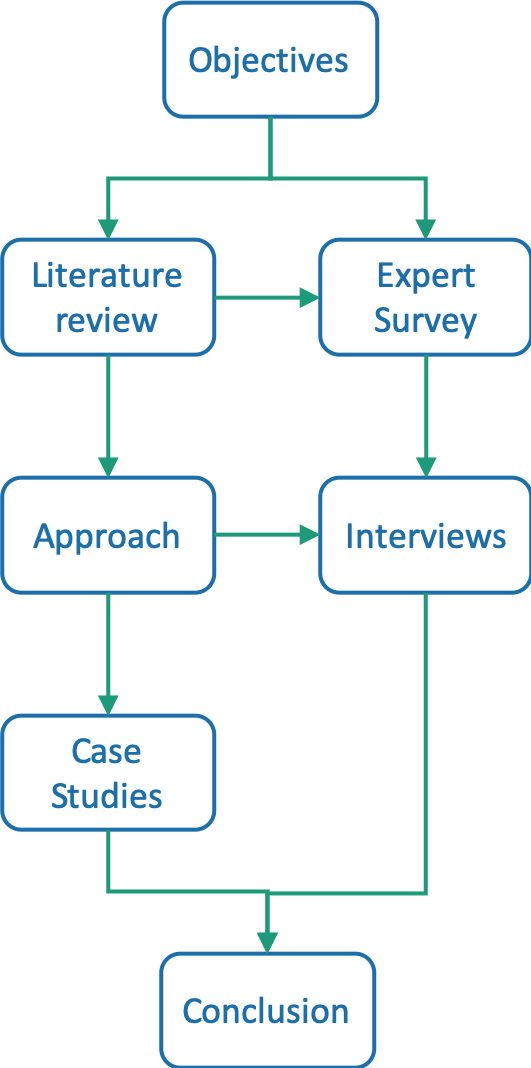
\includegraphics[width=0.5\textwidth]{graphics/thesis-structure}
\caption{Thesis structure}
\label{fig:thesis-structure}
\end{figure}

\begin{description}
    \item[\Autoref{cap:background} - Background]
Here's the literature review.

    \item[\Autoref{cap:thesis_objectives} - Thesis Objectives]
We define the objectives of our work.

...

    \item[\Autoref{cap:conclusion} - Conclusion]
In the last chapter, we discuss our results obtained ...

\end{description}



% Related work 
\chapter{Notations}
Consider a simple, non-empty Graph $G = (V, E)$ comprising a set of Edges $E$ and vertices $E$.
For specificity, $E(G)$ and $V(G)$ is used to refer to the set of edges and vertices associated
with Graph $G$ respectively, where required.Further, denote by $|V|$ the cardinality of set of
vertices $V$, let $G$ be a Graph with $|V(G)| = |\{v_1, v_2, \ldots, v_n \}| = n$ vertices and
$|E(G)| = m$ edges with $E \subset \binom{V}{2} $;
where $\binom{V}{2} = \left\{\left\langle u,v\right\rangle | u,v \in V, u \neq v \right\} $, that is,
the set of all possible unordered pairs created from $V$. For each $e = \left\langle u, v\right\rangle \in E$,
$e$ is said to be incident on $u,v\in V$, whereas $u$ and $v$ are adjacent to each other.

The Neighbor set $\mathcal{N}(v)$ of $v \in V$, defined as
$\mathcal{N}(v) =: \left\{w  \in V(G) | v \neq w, \exists e \in E(G)\right\} $  is the set of vertices
(other than $v$) adjacent to $v \tilde{\mathcal{V}}  \bar{\mathcal{V}}$. Given a Graph $\mathcal{G}$,
$\mathcal{G} \subseteq G$ denotes that $\mathcal{G}$ is a subgraph of $G$, if it holds that
$\forall e \in E(\mathcal{G}),  \; u,v \subseteq V(\mathcal{G})$, $V(\mathcal{G}) \subseteq V(G)$
and $E(\mathcal{G}) \subseteq E(G)$.

The adjacency matrix of a weighted graph $G$ is a symmetric matrix $A \in \mathbb{R}^{n \times n}$ with $i$th row and $j$th
column containing the number of edges incident on vertex $v_i$ and $v_j$. More precisely,
let $\omega : \left\{ 0,1 \right\} \mapsto \mathbb{R}^+_0$ for $i,j \in \left\{1,2, \ldots, n \right\} $

\begin{equation}\label{eqn: adj_matrix}
  A_{i,j} = \begin{cases}
    \omega (e_i), & \qquad e_i = \left\langle v_i, v_j\right\rangle \in E(G) \\
    0,            & \qquad \text{otherwise.}
  \end{cases}
\end{equation}
By restricting \eqref{eqn: adj_matrix} $\omega \in \left\{ 0,1 \right\} \;\forall  \omega  (e_i), \; e_i  \in E$, we recover the
adjacency matrix of an unweighted graph. The volume $vol(F)$ of a a subset of nodes $F \in V$ is the sum of weight of edges adjacent
to the nodes of $F$ and given as $vol(F) = \sum_{v_i \in F}  \delta(v_i)$; where $\delta(v_i)$ is the degree of vertex $v_i$ obtained
as the sum of the weights of edges incident on it: $\delta(v_i) = \sum_{i = 1}^{n} A_{i,j} $.

Denote the number of components in of graph $G$ by $\kappa(G)$. For the a set $V^* \subseteq V(G)$, $V^*$ is a cut-vertex
if $\kappa(G[V(G)\backslash V^* = \tilde{V} ]) > \kappa(G)$; where  $G[\tilde{V}]$ is the graph induced by $\tilde{V}$

\begin{question}[Node Selection]
  \label{pythagorean}
  Is it possible to ensure that the selection of critical nodes in the network is based on both articulation points and their respective changing weights?
  (Where the weight on each critical (or cut) node is the total amount of traffic load generated from non-articulation points).
\end{question}

\begin{approach}
  We would have two optimization objectives base on:
  \begin{enumerate}
    \item maximum volume
    \item cut vertices.
  \end{enumerate}
\end{approach}


\begin{problem}
Given a Graph $G = (V, E)$, let $ \tilde{V} = V(G)\backslash V^*$. Denote by $\vartheta (G)$ the set of cut-vertices associated with Graph $G$ defined by
\begin{equation}
  \vartheta (G) =\left\{(v_i, v_j)\in V^* \; \vert \; \kappa(G[\tilde{V} ]) > \kappa(G)\right\}.
\end{equation}
Further, let the set $\vartheta (\tilde{G} )$ partition  $\vartheta (G)$, that is,
$\vartheta (\tilde{G}) = \bigcup_{i=1}^n \vartheta (G_i)$ where each  $\vartheta (G_i)$ represents each
vertex-cut associated with $\vartheta (G)$. The traffic on $\vartheta (G_i)$ is represented by its volume
of edges $e \in E(G)$
incident on it and expressed as
\begin{equation}
  vol(\vartheta (G_i)) = \sum_{\vartheta (G_i)\in G} \delta(\vartheta (G_i))
\end{equation}

\end{problem}

% Related work 
\chapter{Related Work}
...
\cleardoublepage
...


% Method
\chapter{Method}
Here is a sentence, and you can see a nice picture in Figure \ref{fig:brayford}.

\begin{figure}[h]
    \centering
    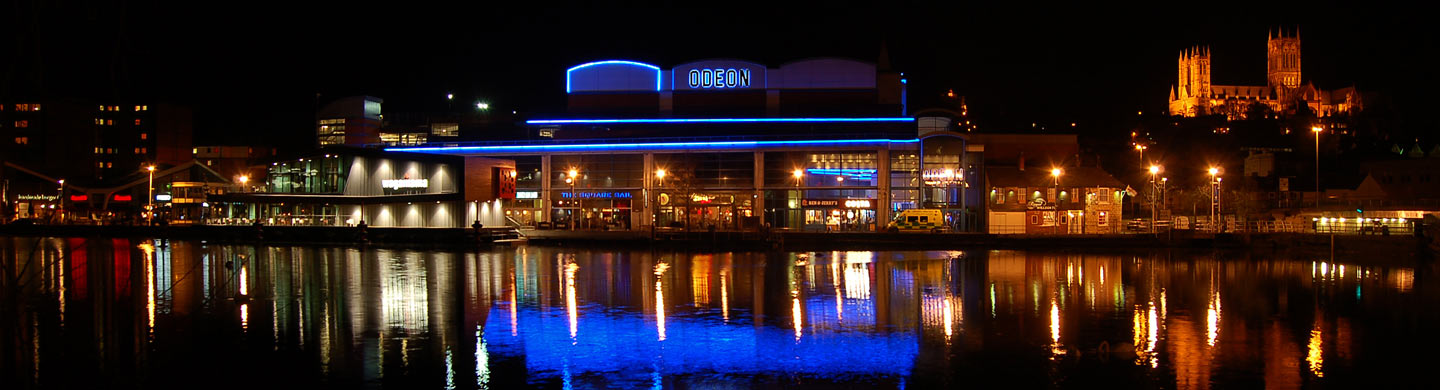
\includegraphics[width=\textwidth]{figures/brayford.jpg}
    \caption{A picture of the Brayford from Google Images.}
    \label{fig:brayford}
\end{figure}

Also, a table can be found in Table \ref{tbl:example-table}. You should use a \LaTeX~table generator like \url{https://www.tablesgenerator.com/} if you want to make your life easier.

\begin{table}[h]
    \caption{Here is a table. The caption goes above like this.}
    \centering
    \begin{tabular}{l|l|c}
        First name & Last name & Age \\
        \hline\hline
        Bob & Bobbington & 24 \\
        Benth & Wavies & 49 \\
        Joe & Bloggs & 37 \\
        Billy & Bob & 10 \\

    \end{tabular}
    \label{tbl:example-table}
\end{table}

% Conclusions
\chapter{Conclusions}
...


% end of thesis body
% --------------------------

% Print out the references
\printReferences

% Print out the ludography (optional)
\printLudography

% If you want to put some text before the list of games,
% then you can use the following code:
%\begin{ludography}[Ludography / Optional Title]
%Here are some games.
%\end{ludography}


\end{document}
